% !TEX root = ../../../main.tex
% 来源：中学数学实验教材·第三册（高中数学）
% 章节：直线、平面坐标化 / 直线坐标化
% 原始文件：2.tex，行 103-130
% 类型：tikz
% ---
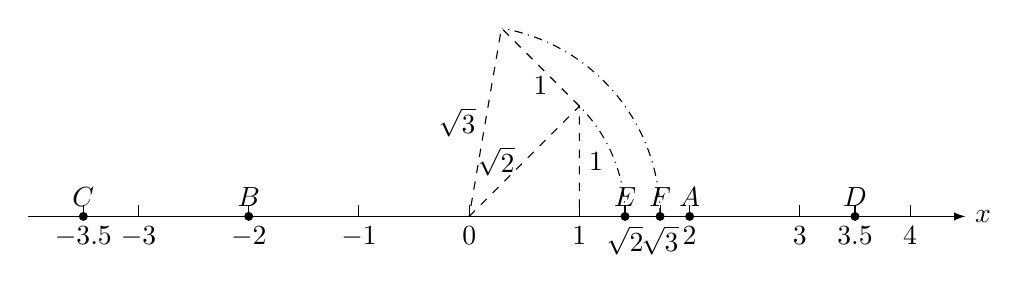
\begin{tikzpicture}[>=latex, scale=1.4]
\draw[->] (-4,0)--(4.5,0) node[right]{$x$};
\foreach \x/\xtext in {2/A,-2/B,-3.5/C,3.5/D,1.414/E,1.732/F}
{
    \draw (\x,0)--(\x,.1);
    \draw (\x,0)[fill=black] circle (1pt);
    \node at (\x,0) [above]{$\xtext$};
}

\foreach \x in {2,-2,-3.5,3.5}
{
    \node at (\x,0) [below]{$\x$};
}

\foreach \x in {-3,-1,0,1,3,4}
{
    \draw (\x,0)--(\x,.1);
    \node at (\x,0) [below]{$\x$};
}
\node at (1.414,0)[below]{$\sqrt{2}$};
\node at (1.732,0)[below]{$\sqrt{3}$};

\draw[dashed] (0,0)--node[left]{$\sqrt{2}$}(1,1)--node[right]{1}(1,0);
\draw[dashdotted] (1.414,0) arc (0:45:1.414);

\draw[dashed]  (1,1)--node[below]{1}(1-1/1.414, 1+1/1.414)--node[left]{$\sqrt{3}$}(0,0);
\draw[dashdotted] (1.732,0) arc (0:80:1.732);
\end{tikzpicture}
